This assignment is about 2-dimensional vectors. A 2-dimensional vector or just a vector is a geometrical object consisting of a direction and a length. Typically, vectors are represented as a coordinate pair $\vec v  = (x, y)$, where the length and direction is found as
\begin{align}
  \text{len}(\vec v) &= \sqrt{x^2+y^2}
  \\\text{ang}(\vec v) &=\text{atan2}(y, x)
\end{align}
For technical reasons, we here use atan2 instead of the usual atan function. The atan2 function is found in F\# as \lstinline{System.Math.Atan2}, which takes the $(y,x)$ tuple argument. The vector's ends are called its tail and tip, and when the tail is placed in $(0, 0)$, then its tip will be in the  $(x, y)$. Vectors have a number of standard operations on them:
\begin{align}
  \vec v_1 &= (x_1, y_1)
  \\\vec v_2 &= (x_2, y_2)
  \\a \vec v_1 &= (a x_1, a y_1)
  \\\vec v_1 + \vec v_2 &= (x_1+x_2, y_1+y_2)
  \\\vec v_1 \cdot \vec v_2 &= x_1 x_2 +  y_1y_2
\end{align}
Addition can be drawn as shown in \Cref{fig:vectorAddition}.
\begin{figure}
  \centering
  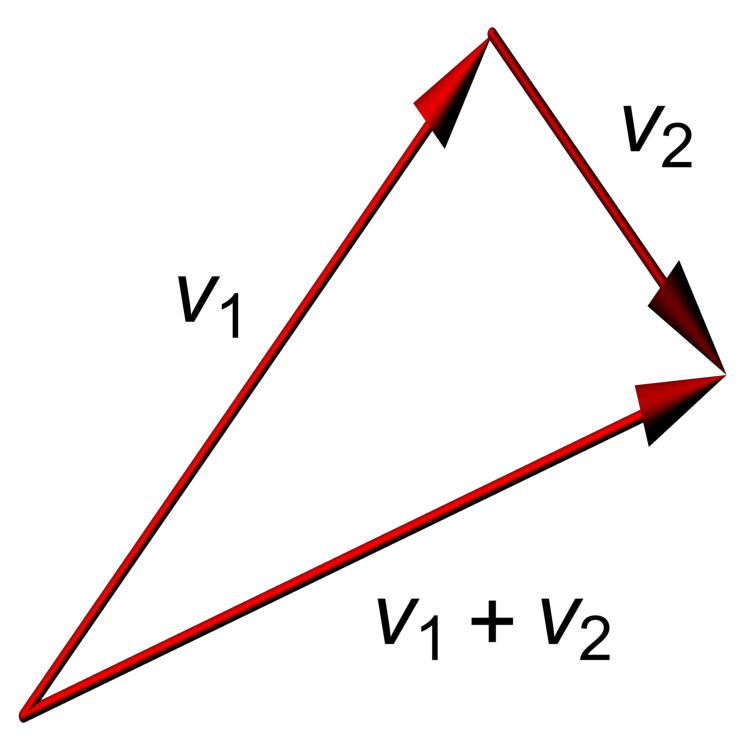
\includegraphics[width=0.28\textwidth]{vectorAddition}
  \caption{Illustration of vector addition in two dimensions.}
  \label{fig:vectorAddition}
\end{figure}
Rotation of a vector by the $a$ counter clockwise and around its tail can be done as,
\begin{equation}
  R_a \vec v_1 = (x\cos(a) - y\sin(a),x\sin(a)+y\cos(a))
\end{equation}
The trigonometric functions are found as \lstinline{System.Math.Cos} and \lstinline{System.Math.Sin}, and they both take an angle in radians as the argument. The constant $\pi$ is found in \lstinline{System.Math.PI}.
